\section{Experiment Result}  \label{sec:experiment_result}

In our comparision, we look at the 11-point interpolation mean average precision (mAP) and 101-point interpolation mAP at 10 different IoU thresholds from 0.5 to 0.95 with the step size of 0.05 (Figure \ref{fig:mrcnn_map} and \ref{fig:yolov5_map}). This configuration is the same of the AP metrics of the COCO benchmarks \cite{coco_2014}. We notice that the $mAP_{11}$ as good of approximation as the $mAP_{101}$ in approximating the area under the precision-recall curve, while $mAP_{11}$ is faster as it require less operations compare to $mAP_{101}$. However, for the remaining of the comparision experiment, we utilize the $mAP_{101}$ as it is more accurate and the evaluation runtime is not important in our comparision software.

We start our experiment with evaluate the Mask R-CNN model performance on the nuImages validation set. When we look at the $mAP_{101}$ at IoU threshold of 0.5, the pretrain Mask R-CNN model is accurate at 51.82\%, signal that the model able to detect human and vehicle more than 50\% of the times without the need of domain training. However, the $mAP_{101}$ score drop significiantly as the IoU threshold increase. This indicate that the region proposal network (RPN) and bounding box regressor are struggling in correctly proposing RoI and finetuning it to align well with the ground-truth object.

\begin{figure}[!ht]
    \centering
    \subfloat[][$mAP_{11}$ and $mAP_{101}$ values]{
        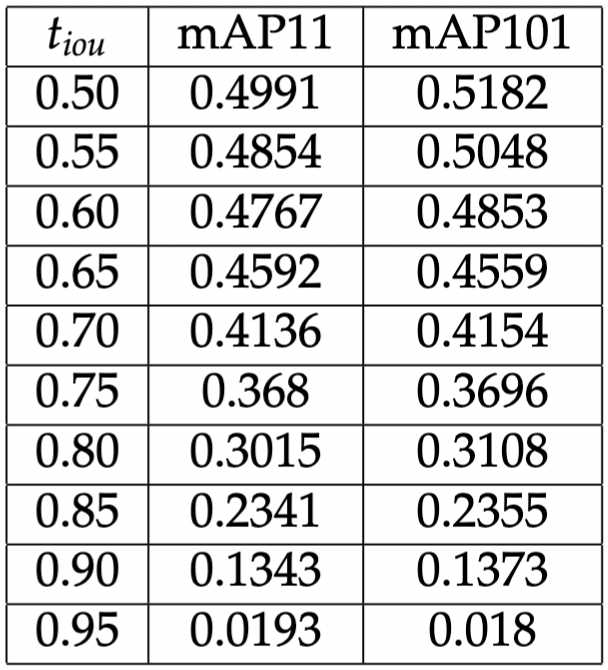
\includegraphics[height=2.25in]{figures/mrcnn_map.png}
    }
    \quad
    \subfloat[][$mAP_{11}$ and $mAP_{101}$ curves]{ 
        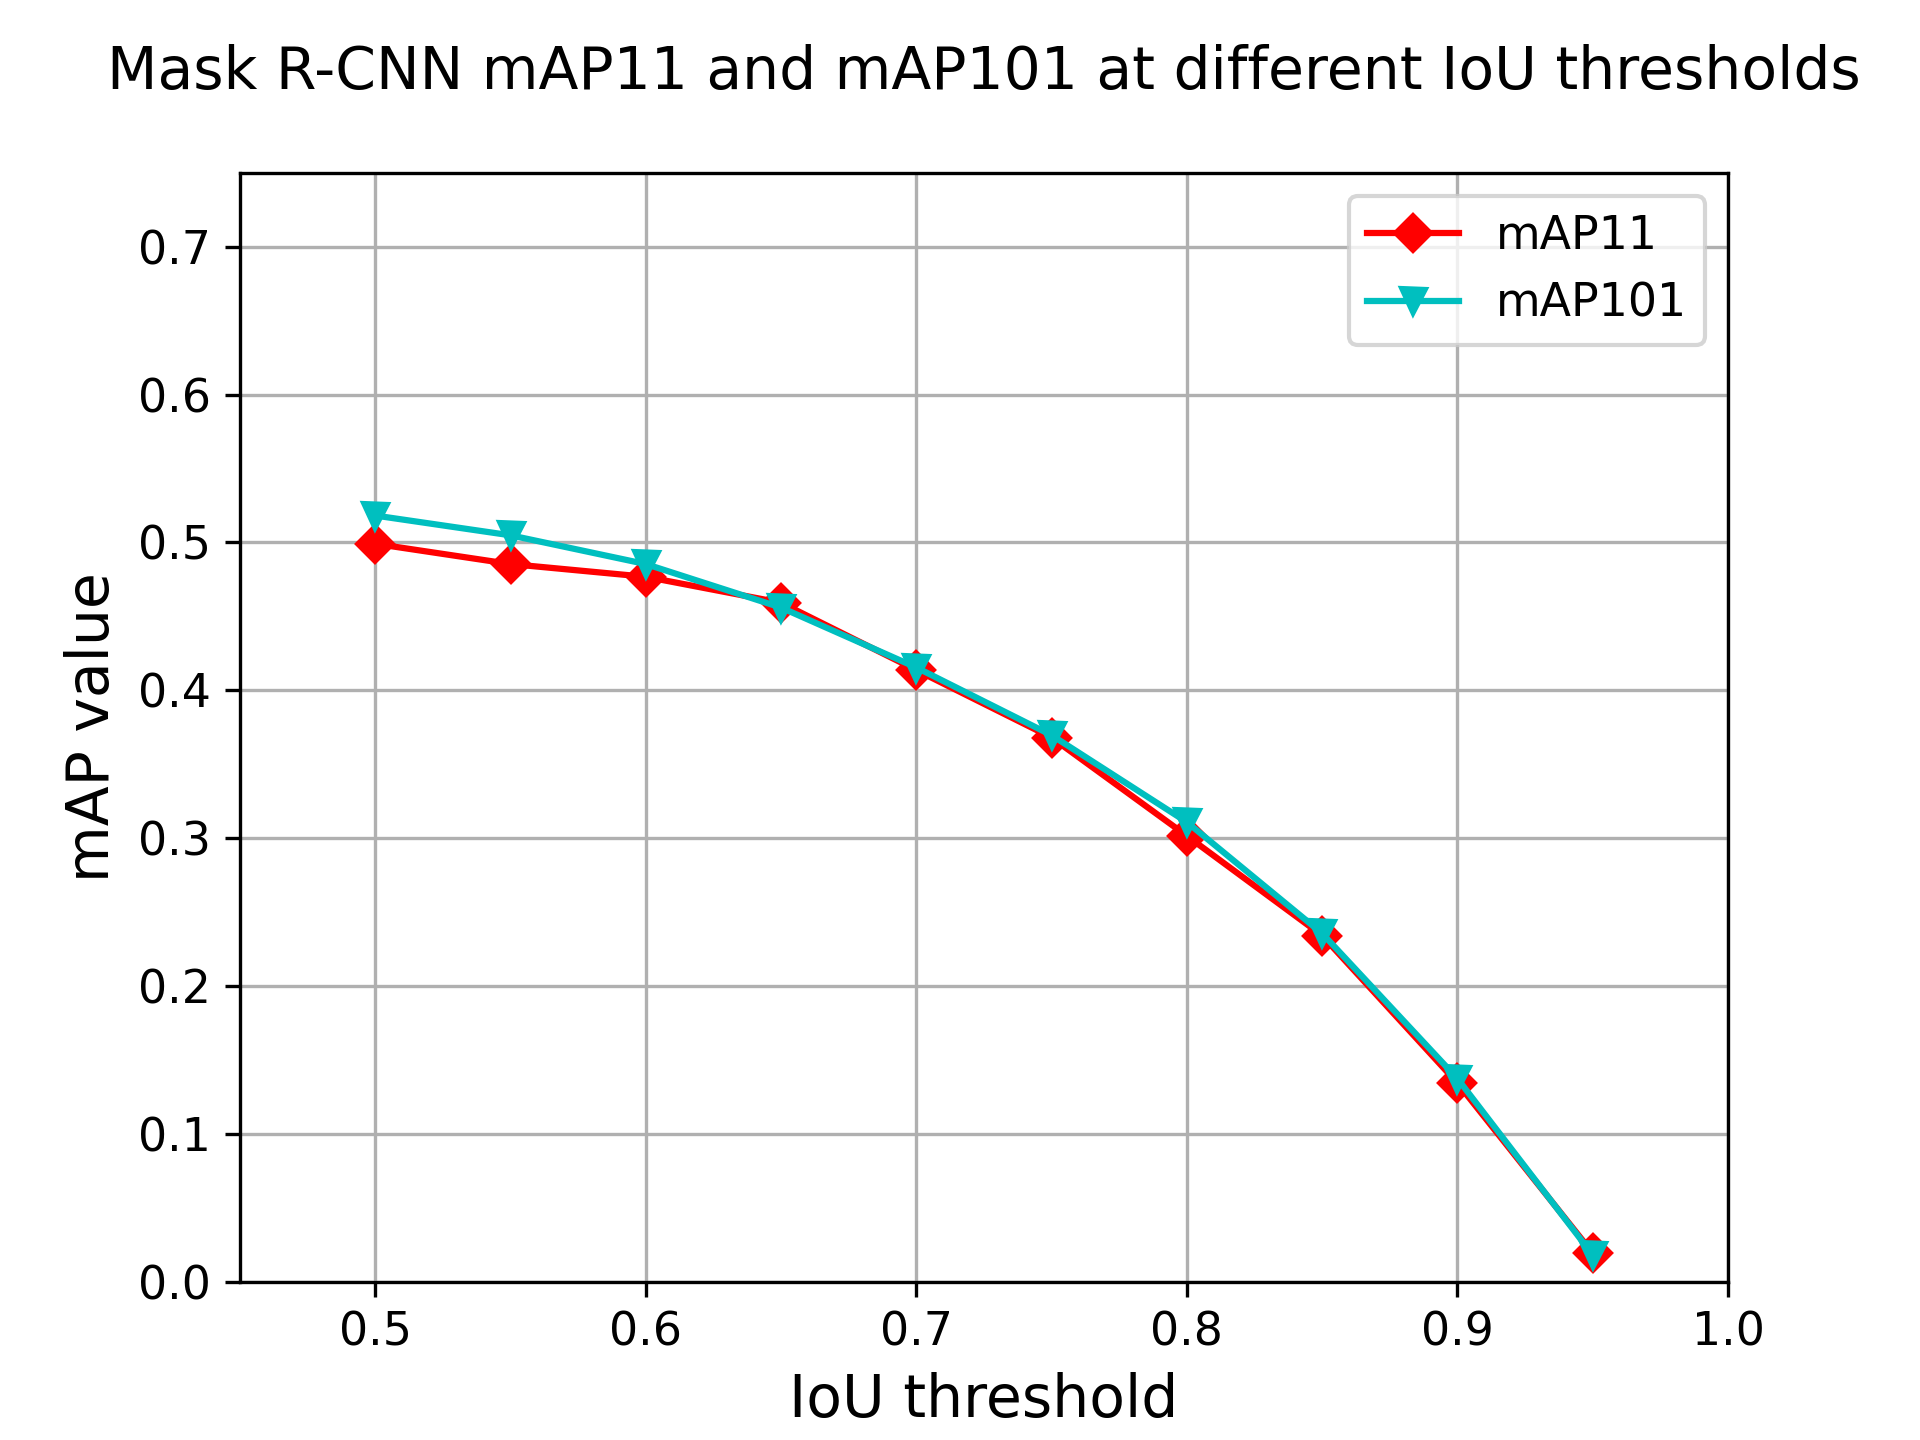
\includegraphics[height=2.25in]{figures/mrcnn_map_curve.png}
    }
    \caption{Mask R-CNN model 11-point interpolation mAP ($mAP_{11}$) and 101-point interpolation mAP ($mAP_{101}$) at different IoU thresholds. The IoU threshold list is defined as [0.5:0.05:0.95], which means the IoU thresholds are from 0.50 to 0.95 with an equal step size of 0.05}  \label{fig:mrcnn_map}
\end{figure}

In constrast to Mask R-CNN, the pretrain YOLOv5 model only have the $mAP_{101}$ score of 47.18\% at IoU threshold of 0.5, which indicate that the model is struggling with able to detect the object present in the image. However, YOLOv5 $mAP_{101}$ score is gradually decrease as we increase the IoU threshold until 0.85. This means that YOLOv5 detector is strong in localization task with majority of predicted bouding box, that has IoU larger than 0.5, will have the IoU score of 0.85 approximately.

\begin{figure}[!ht]
    \centering
    \subfloat[][$mAP_{11}$ and $mAP_{101}$ values]{
        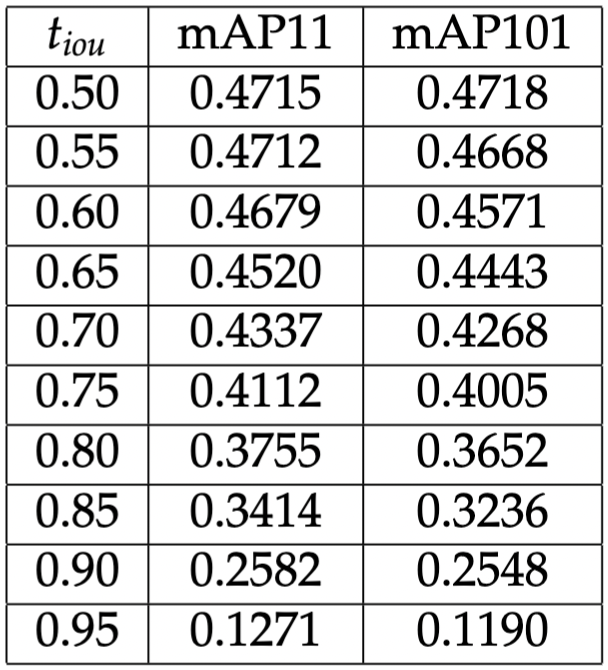
\includegraphics[height=2.25in]{figures/yolov5_map.png}
    }
    \quad
    \subfloat[][$mAP_{11}$ and $mAP_{101}$ curves]{ 
        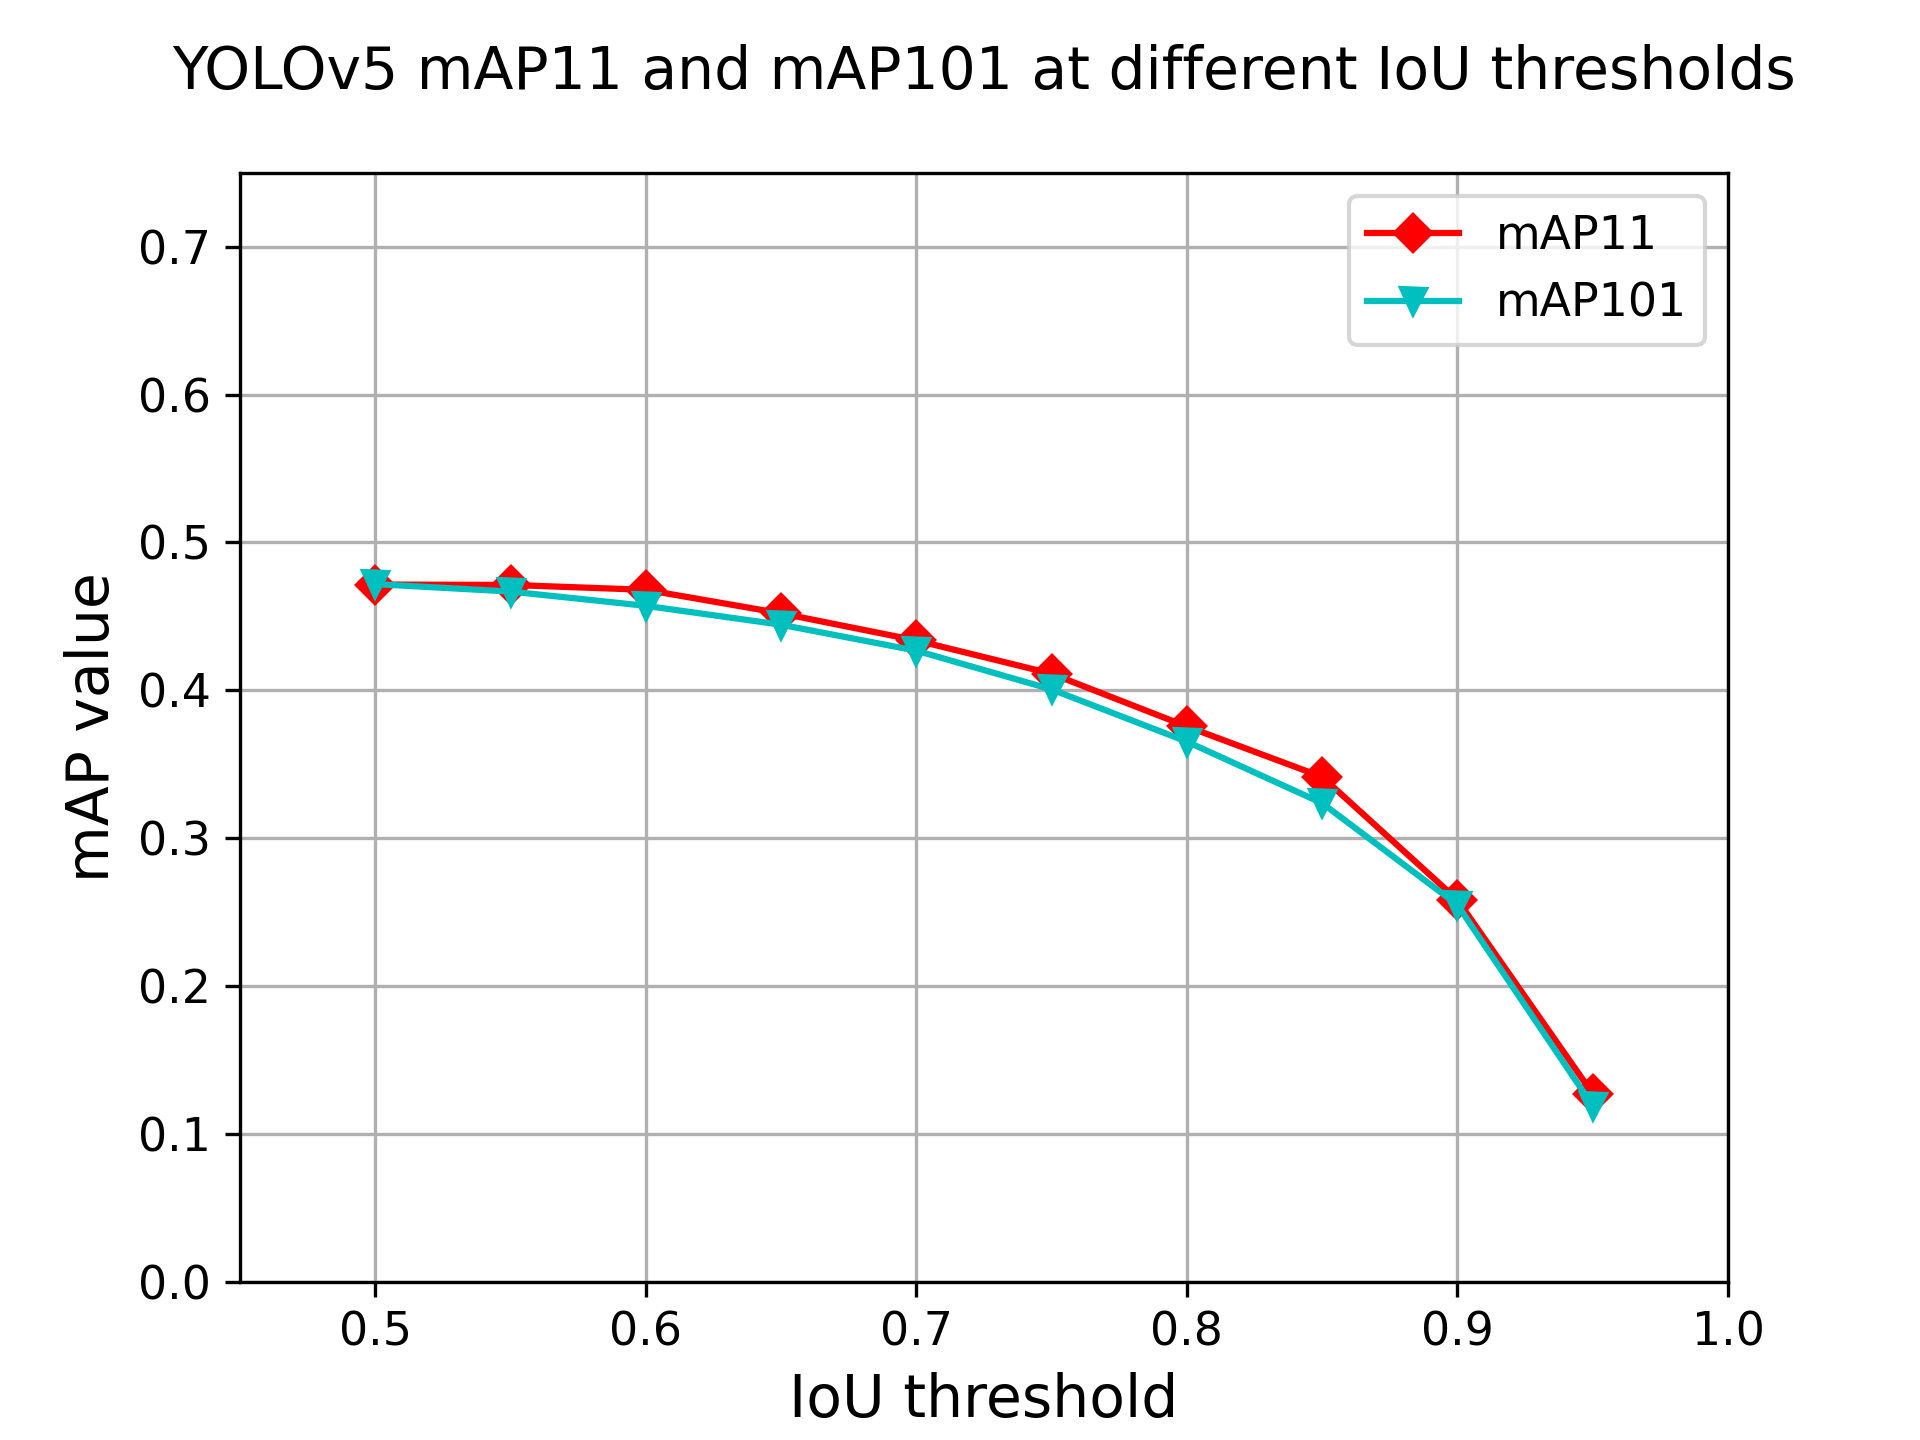
\includegraphics[height=2.25in]{figures/yolov5_map_curve.png}
    }
    \caption{YOLOv5 model 11-point interpolation mAP ($mAP_{11}$) and 101-point interpolation mAP ($mAP_{101}$) at different IoU thresholds. The IoU threshold list is defined as [0.5:0.05:0.95]}  \label{fig:yolov5_map}
\end{figure}

By comparing the $mAP_{101}$ score of the Mask R-CNN and YOLOv5 models, we can clearly see that Mask R-CNN is better at detecting the present of object compare to YOLOv5, however it have a poor localization performance. With poor localization, many detection make by Mask R-CNN is consider as wrong (False Positive) as IoU threshold increase, and thus reduce the overall $mAP_{101}$ score significiantly. On the other hand, YOLOv5, with the high accuracy localization, become a better detection model as the IoU threshold approaching 1 (Firgure \ref{fig:mrcnn_yolov5_map}). Therefore, for autonomous vehicle application where both objectiveness and localization are important, YOLOv5 is a better suited model compare to Mask R-CNN model. In addition to $mAP_{101}$ score, the break down $AP_{101}$ score for each class of the two model at IoU thresholds of 0.55, 0.65, 0.75, and 0.85 is shown in Figure \ref{fig:ap101_perlabel_periou}. Nonetheless, eventhough YOLOv5 is better compare to Mask R-CNN, at IoU threshold of 0.85 and confidence threshold of 0.5, YOLOv5 still unable to detect majority of ground truth object. The visualization of number of missed detection for Mask R-CNN and YOLOv5 model are shown in Figure \ref{fig:model_missed_detection}

\begin{figure}[!ht]
    \centering
    \subfloat[][$mAP_{101}$ values]{
        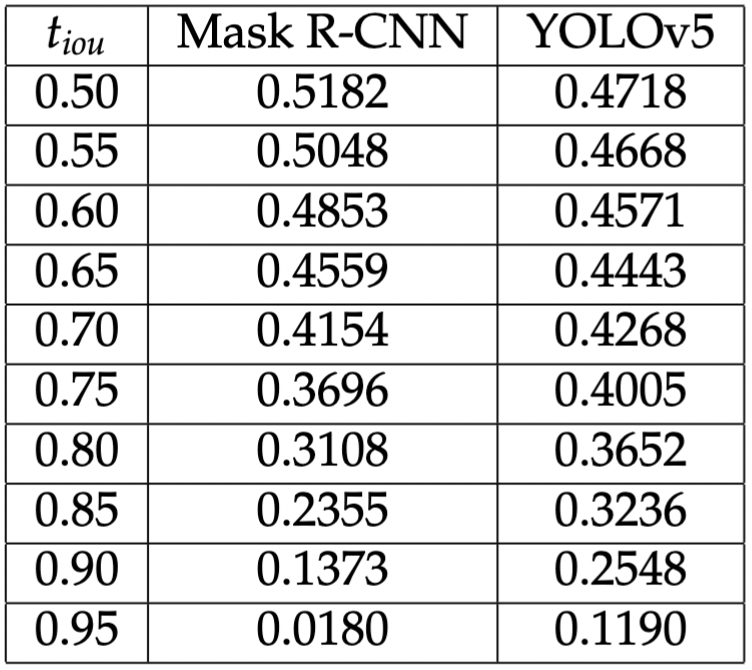
\includegraphics[height=2.25in]{figures/mrcnn_yolov5_map101.png}
    }
    \quad
    \subfloat[][$mAP_{101}$ curves]{ 
        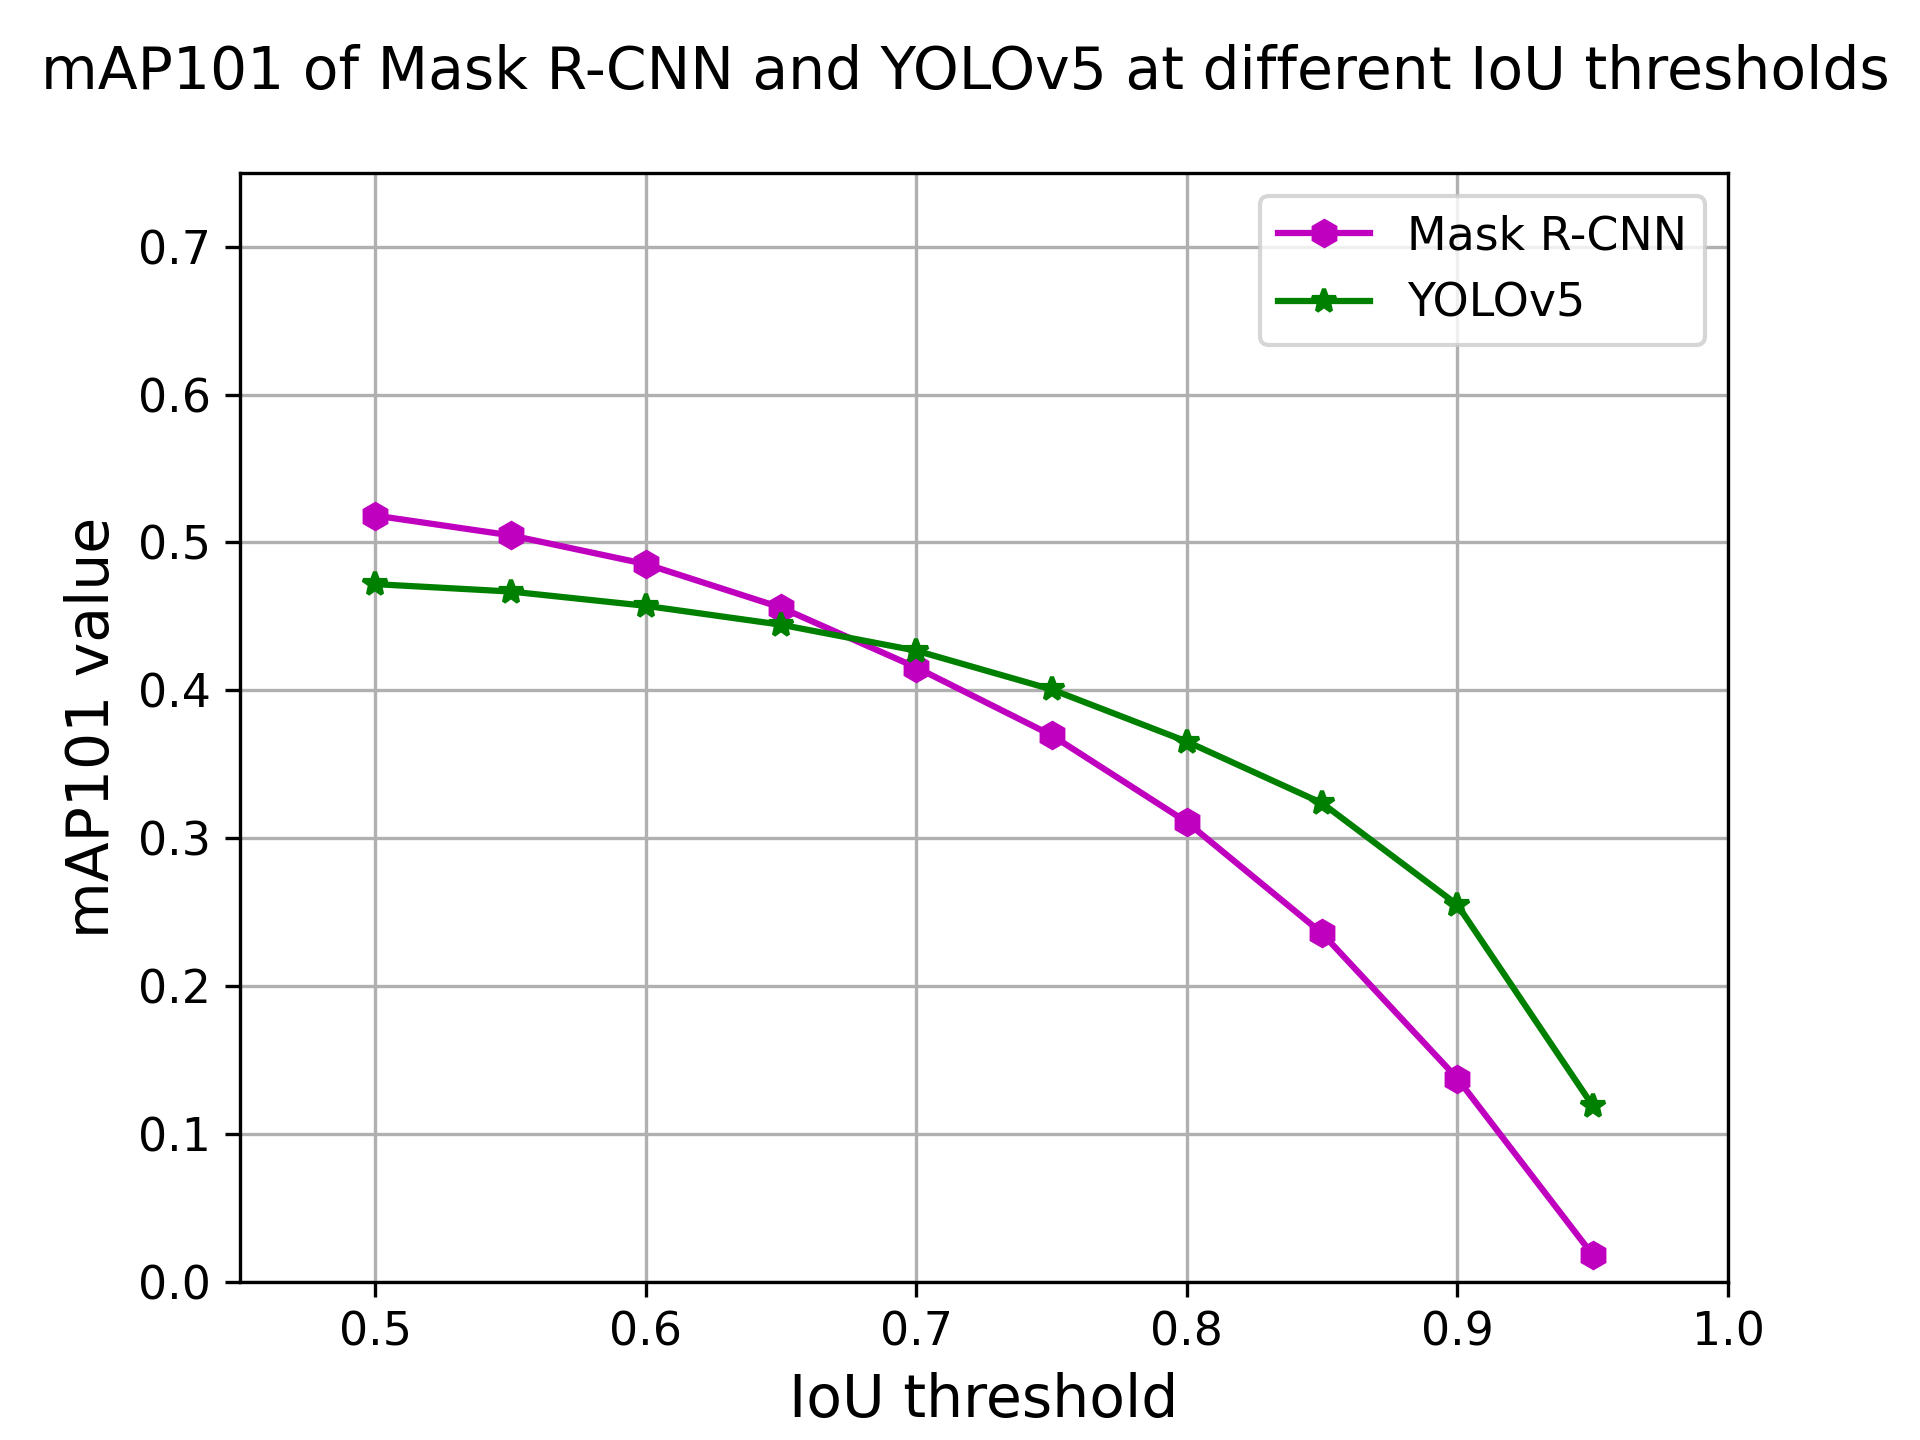
\includegraphics[height=2.25in]{figures/mrcnn_yolov5_map_curve.png}
    }
    \caption{Mask R-CNN's $mAP_{101}$ and YOLOv5's $mAP_{101}$ at different IoU thresholds. The IoU threshold list is defined as [0.5:0.05:0.95]} \label{fig:mrcnn_yolov5_map}
\end{figure}

\begin{figure}[!ht]
    \centering
    \subfloat[][IoU threshold $t_{IoU}=0.55$]{
        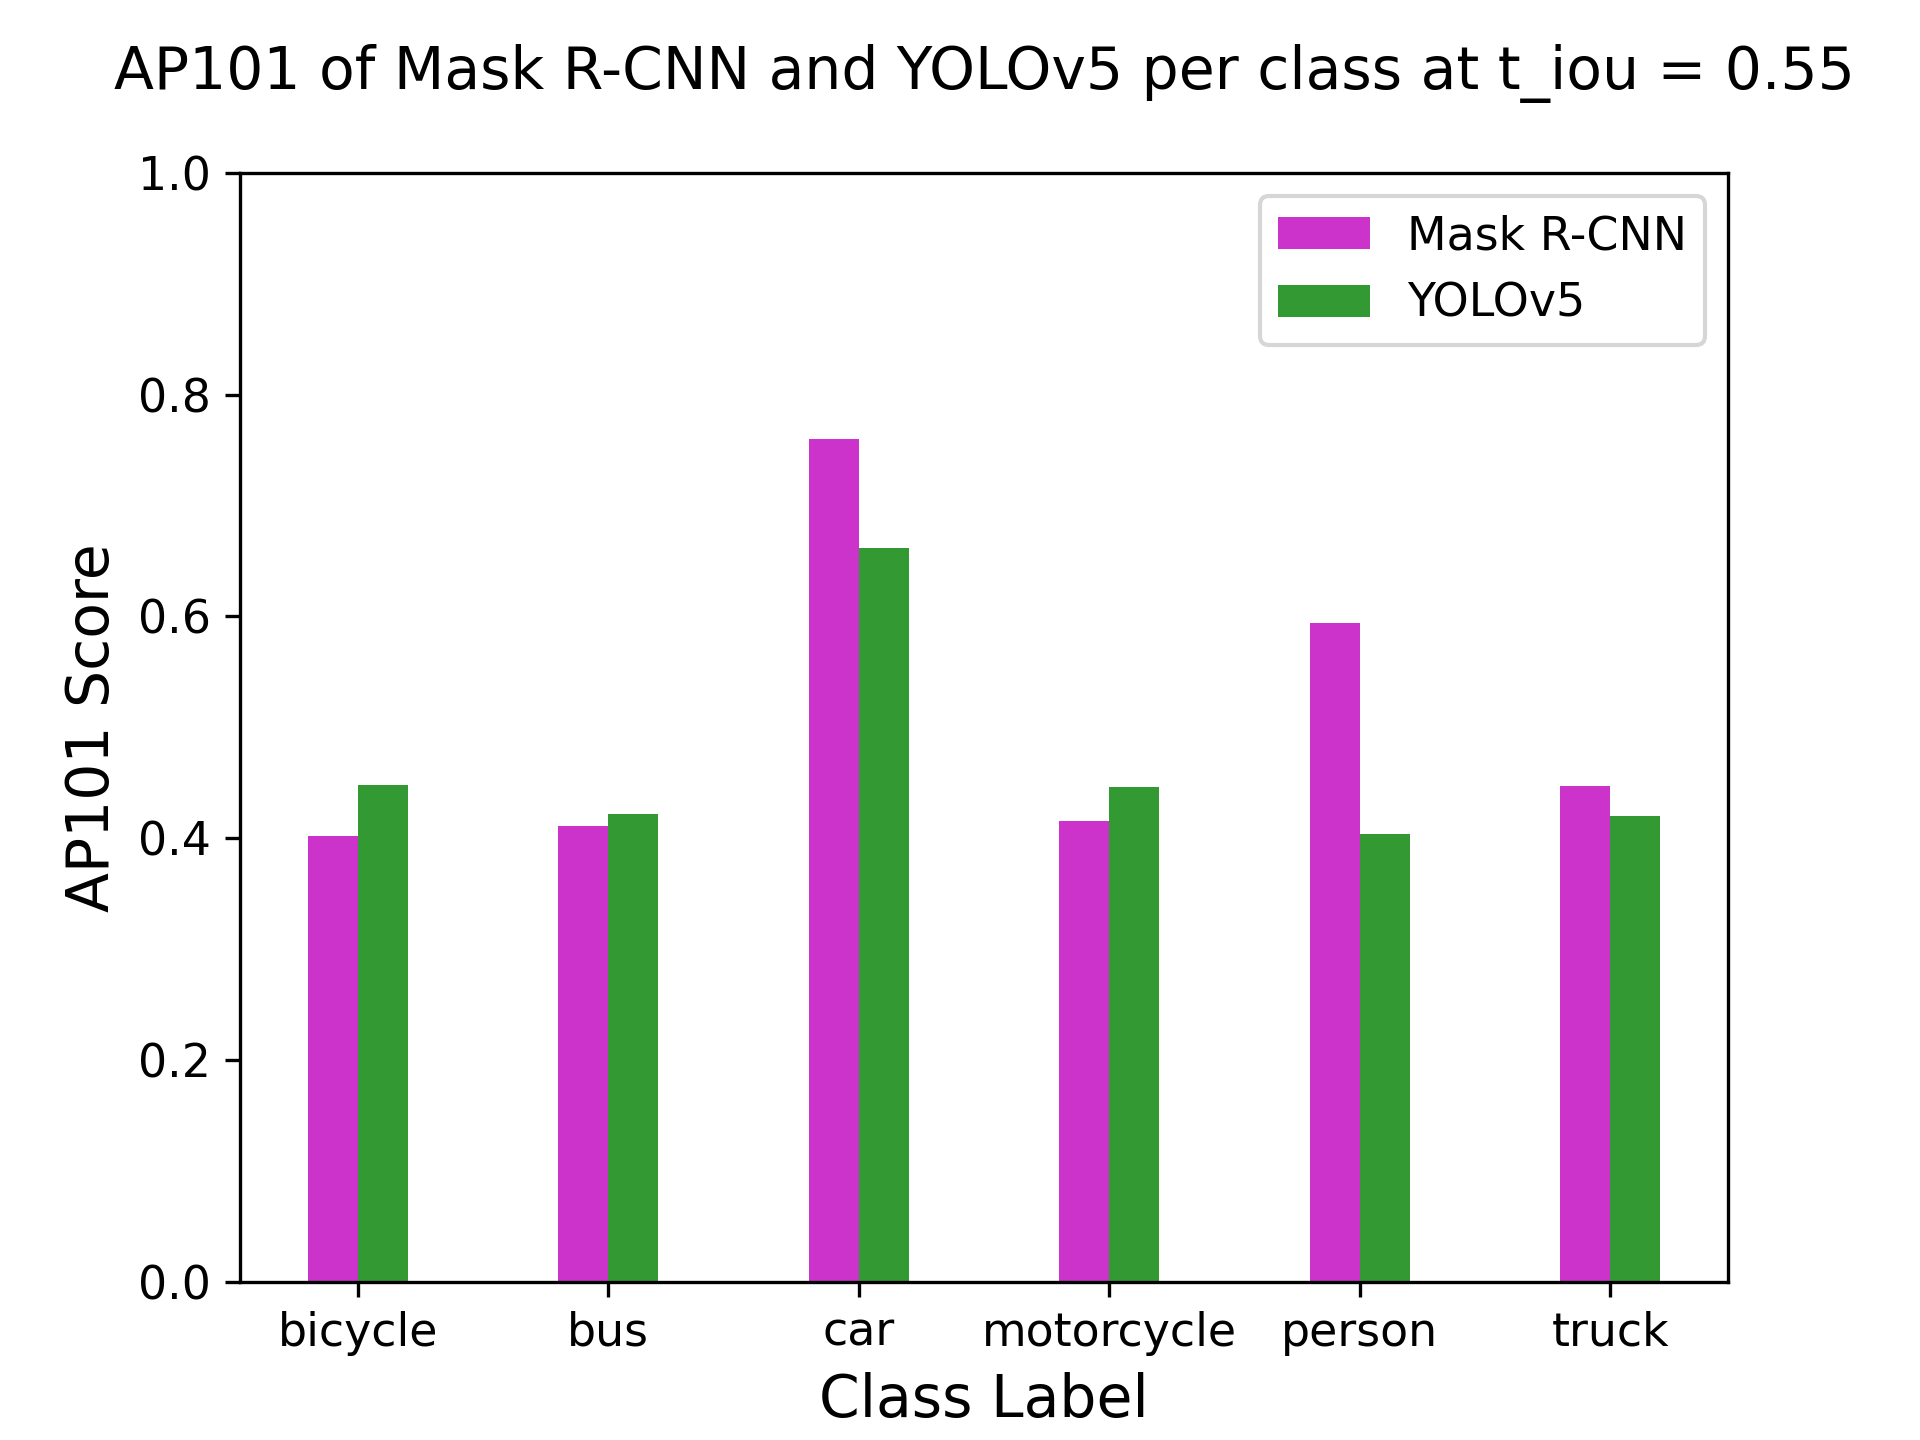
\includegraphics[height=1.5in]{figures/ap101_i55.png}
    }
    \quad
    \subfloat[][IoU threshold $t_{IoU}=0.65$]{
        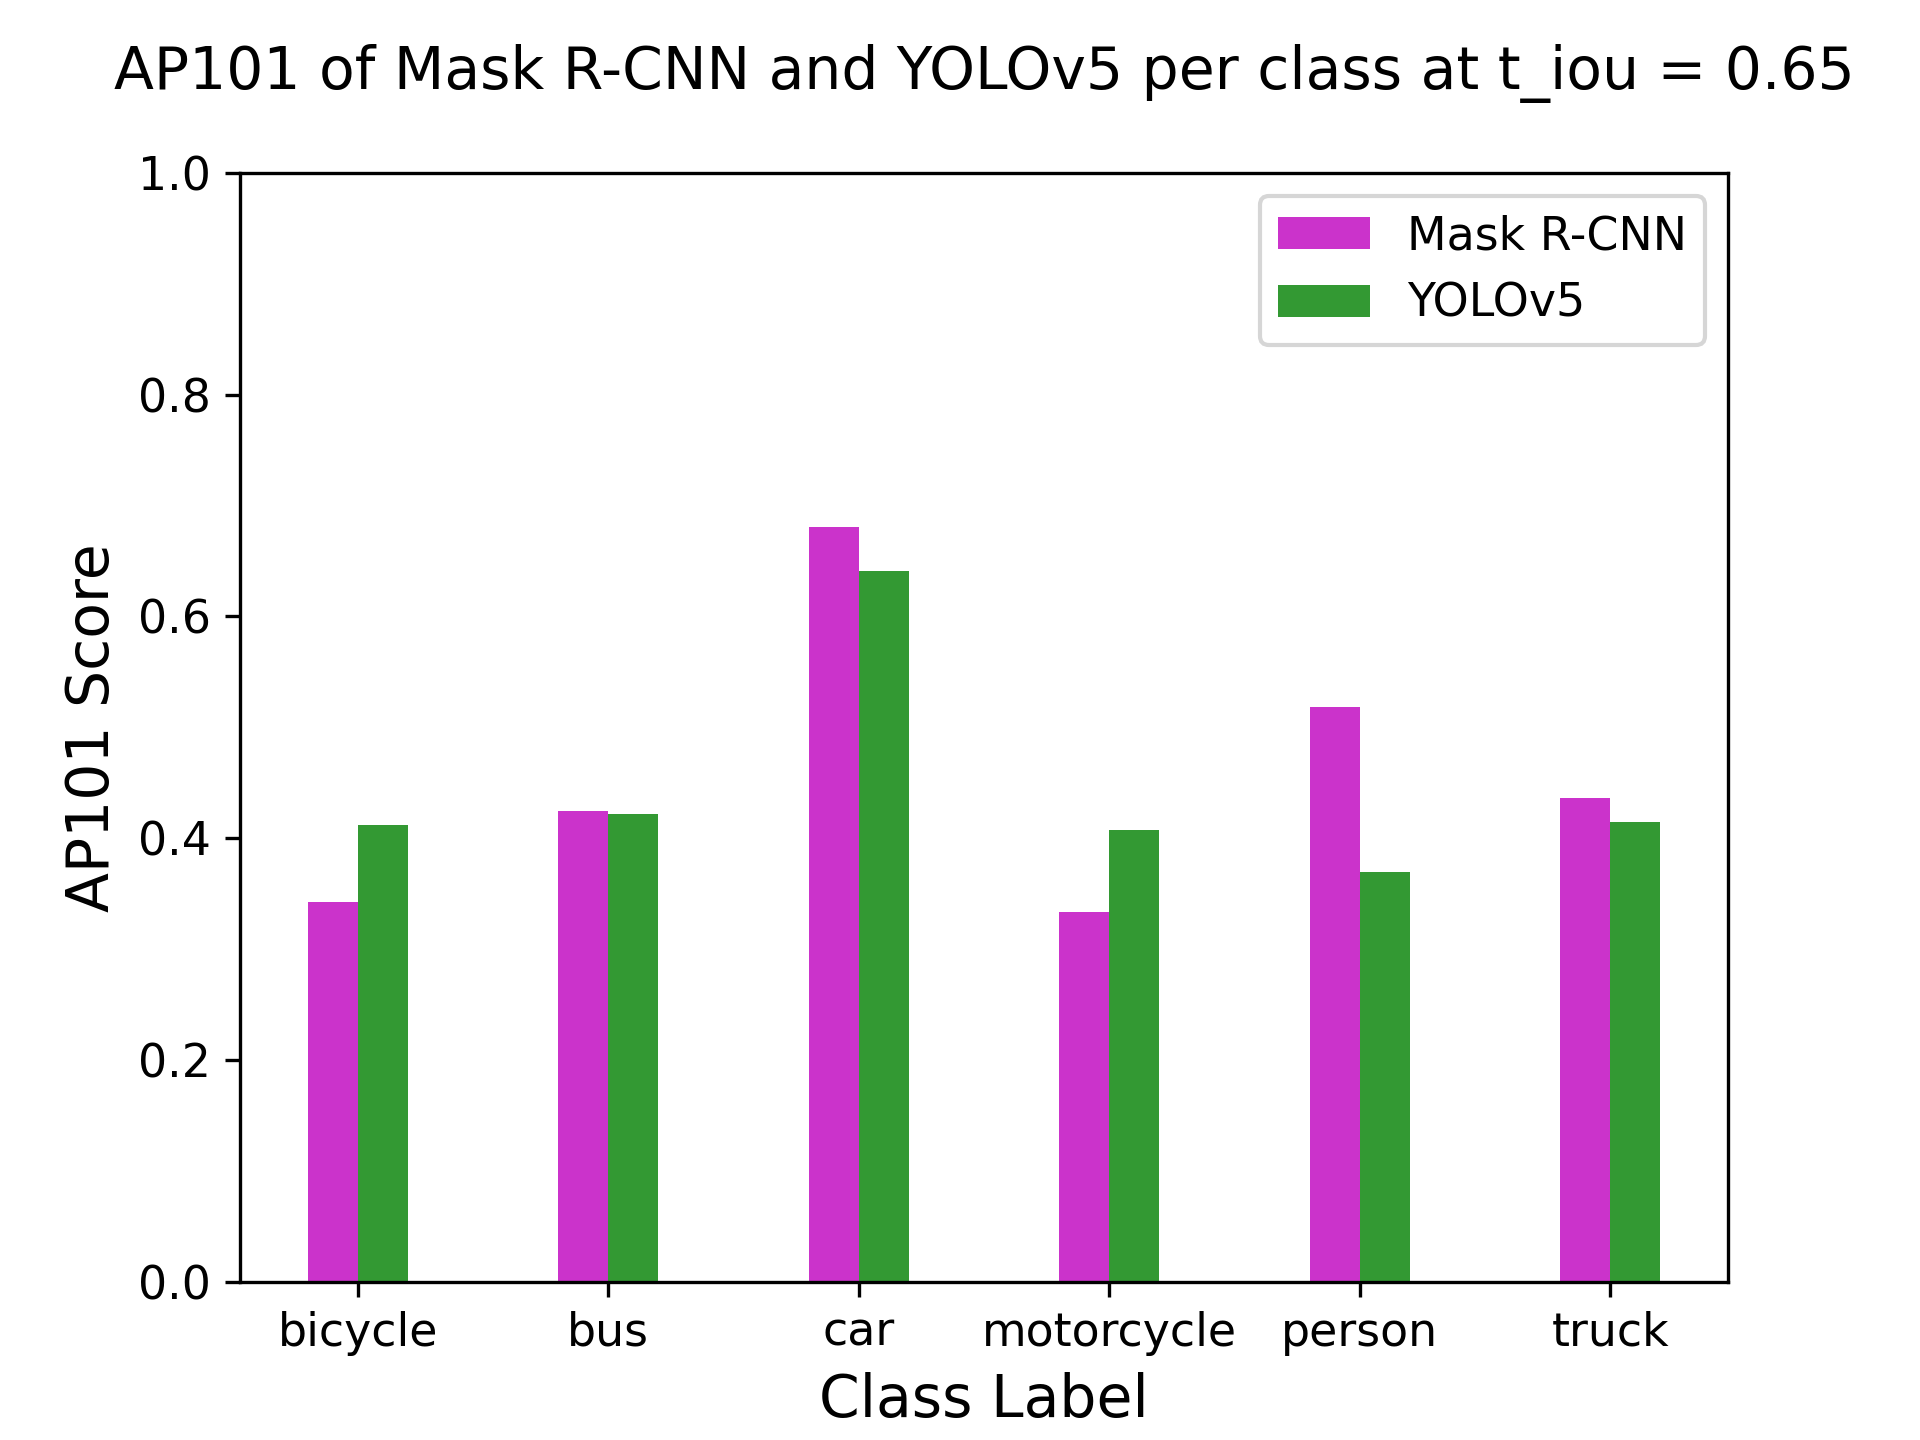
\includegraphics[height=1.5in]{figures/ap101_i65.png}
    }

    \subfloat[][IoU threshold $t_{IoU}=0.75$]{
        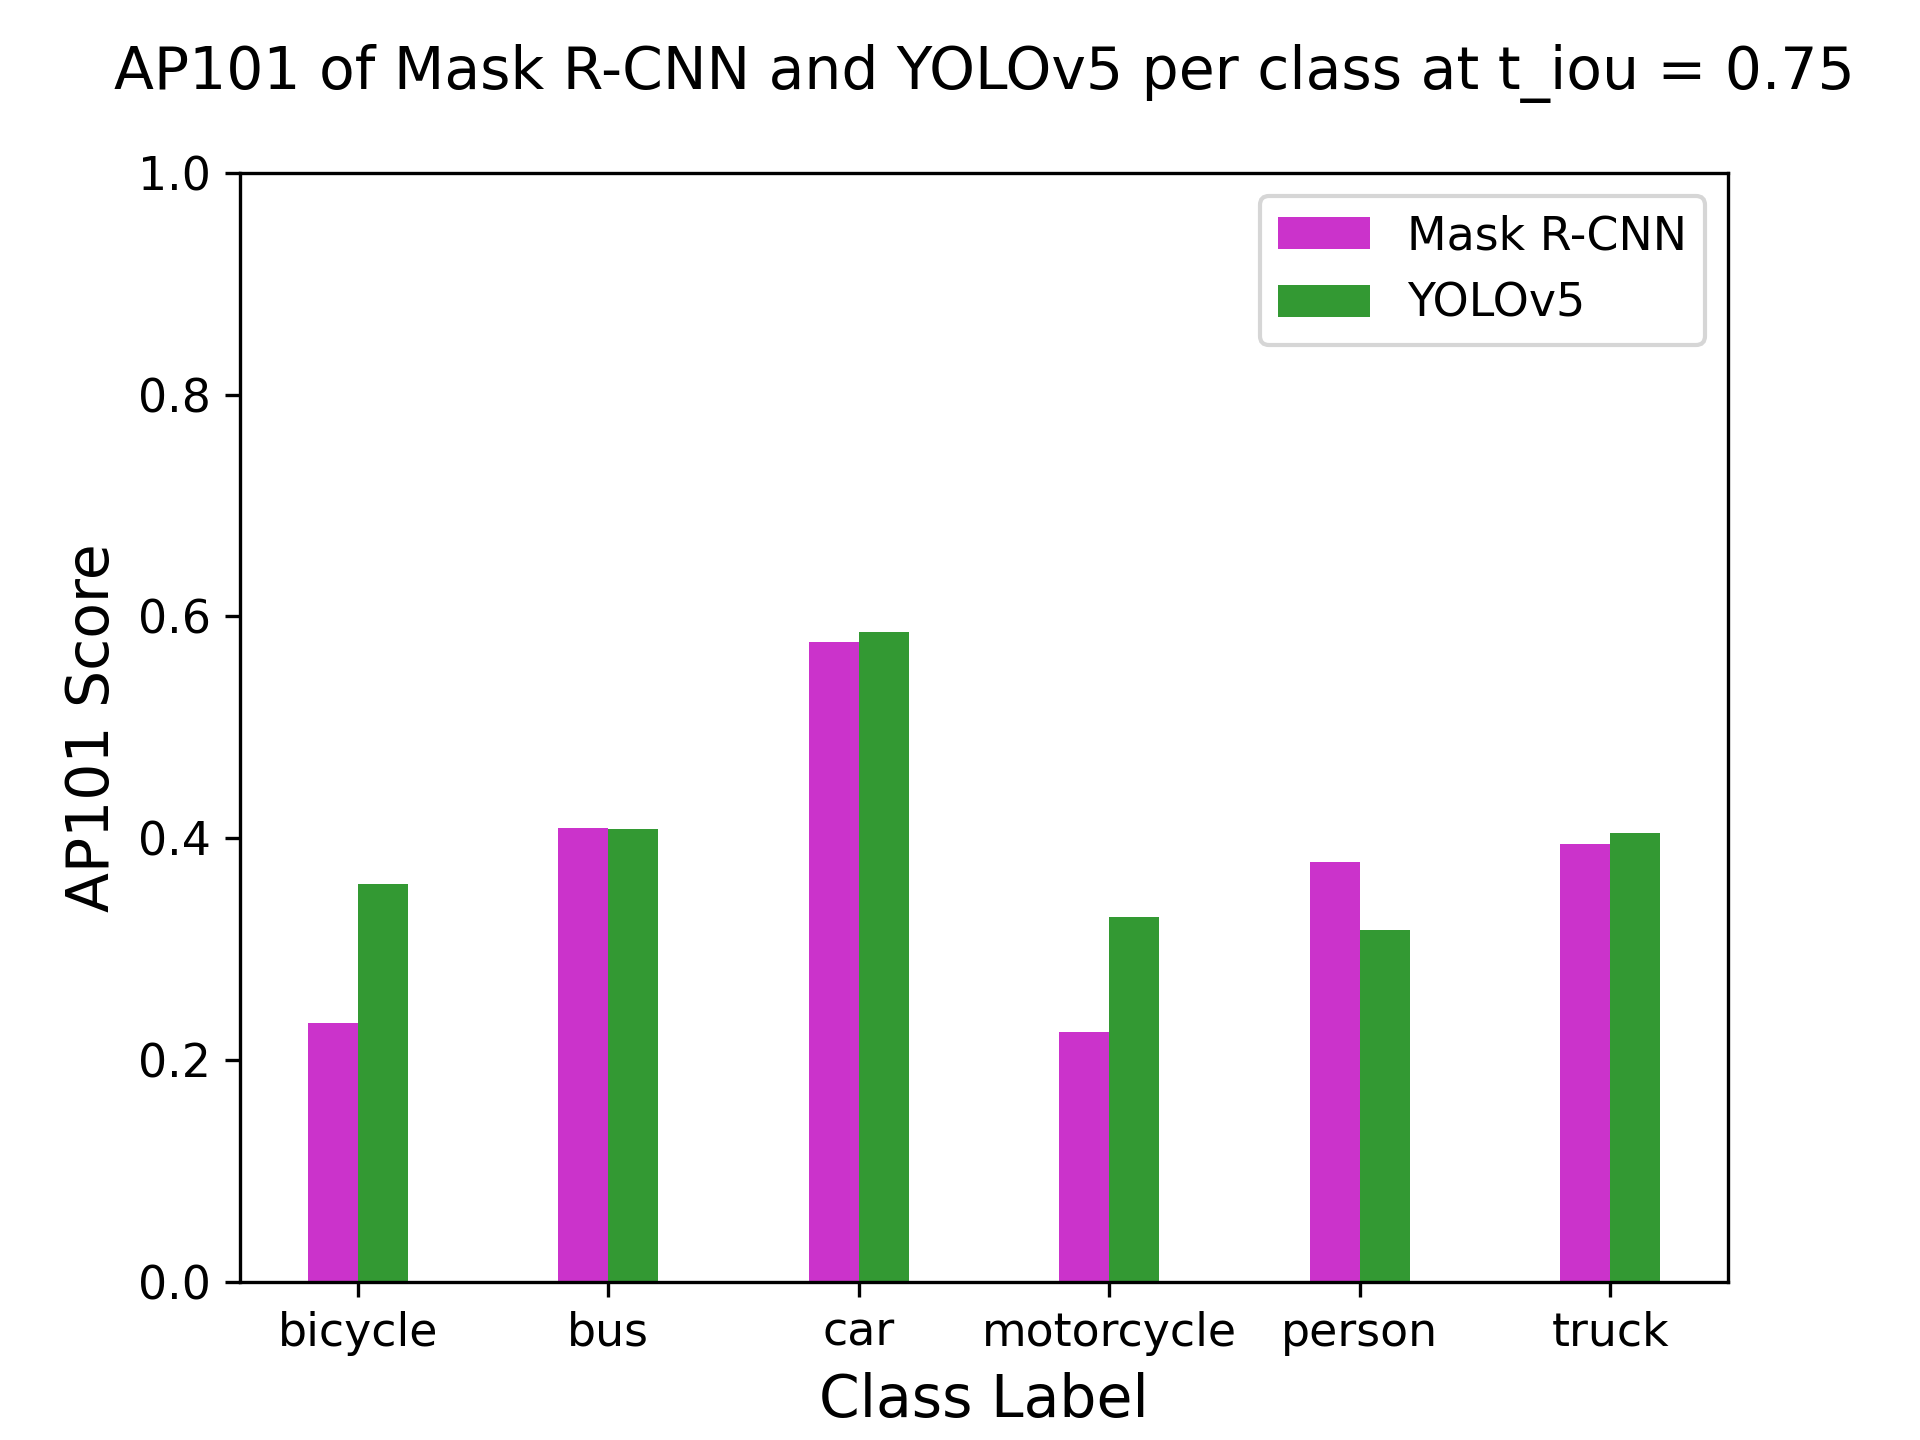
\includegraphics[height=1.5in]{figures/ap101_i75.png}
    }
    \quad
    \subfloat[][IoU threshold $t_{IoU}=0.85$]{
        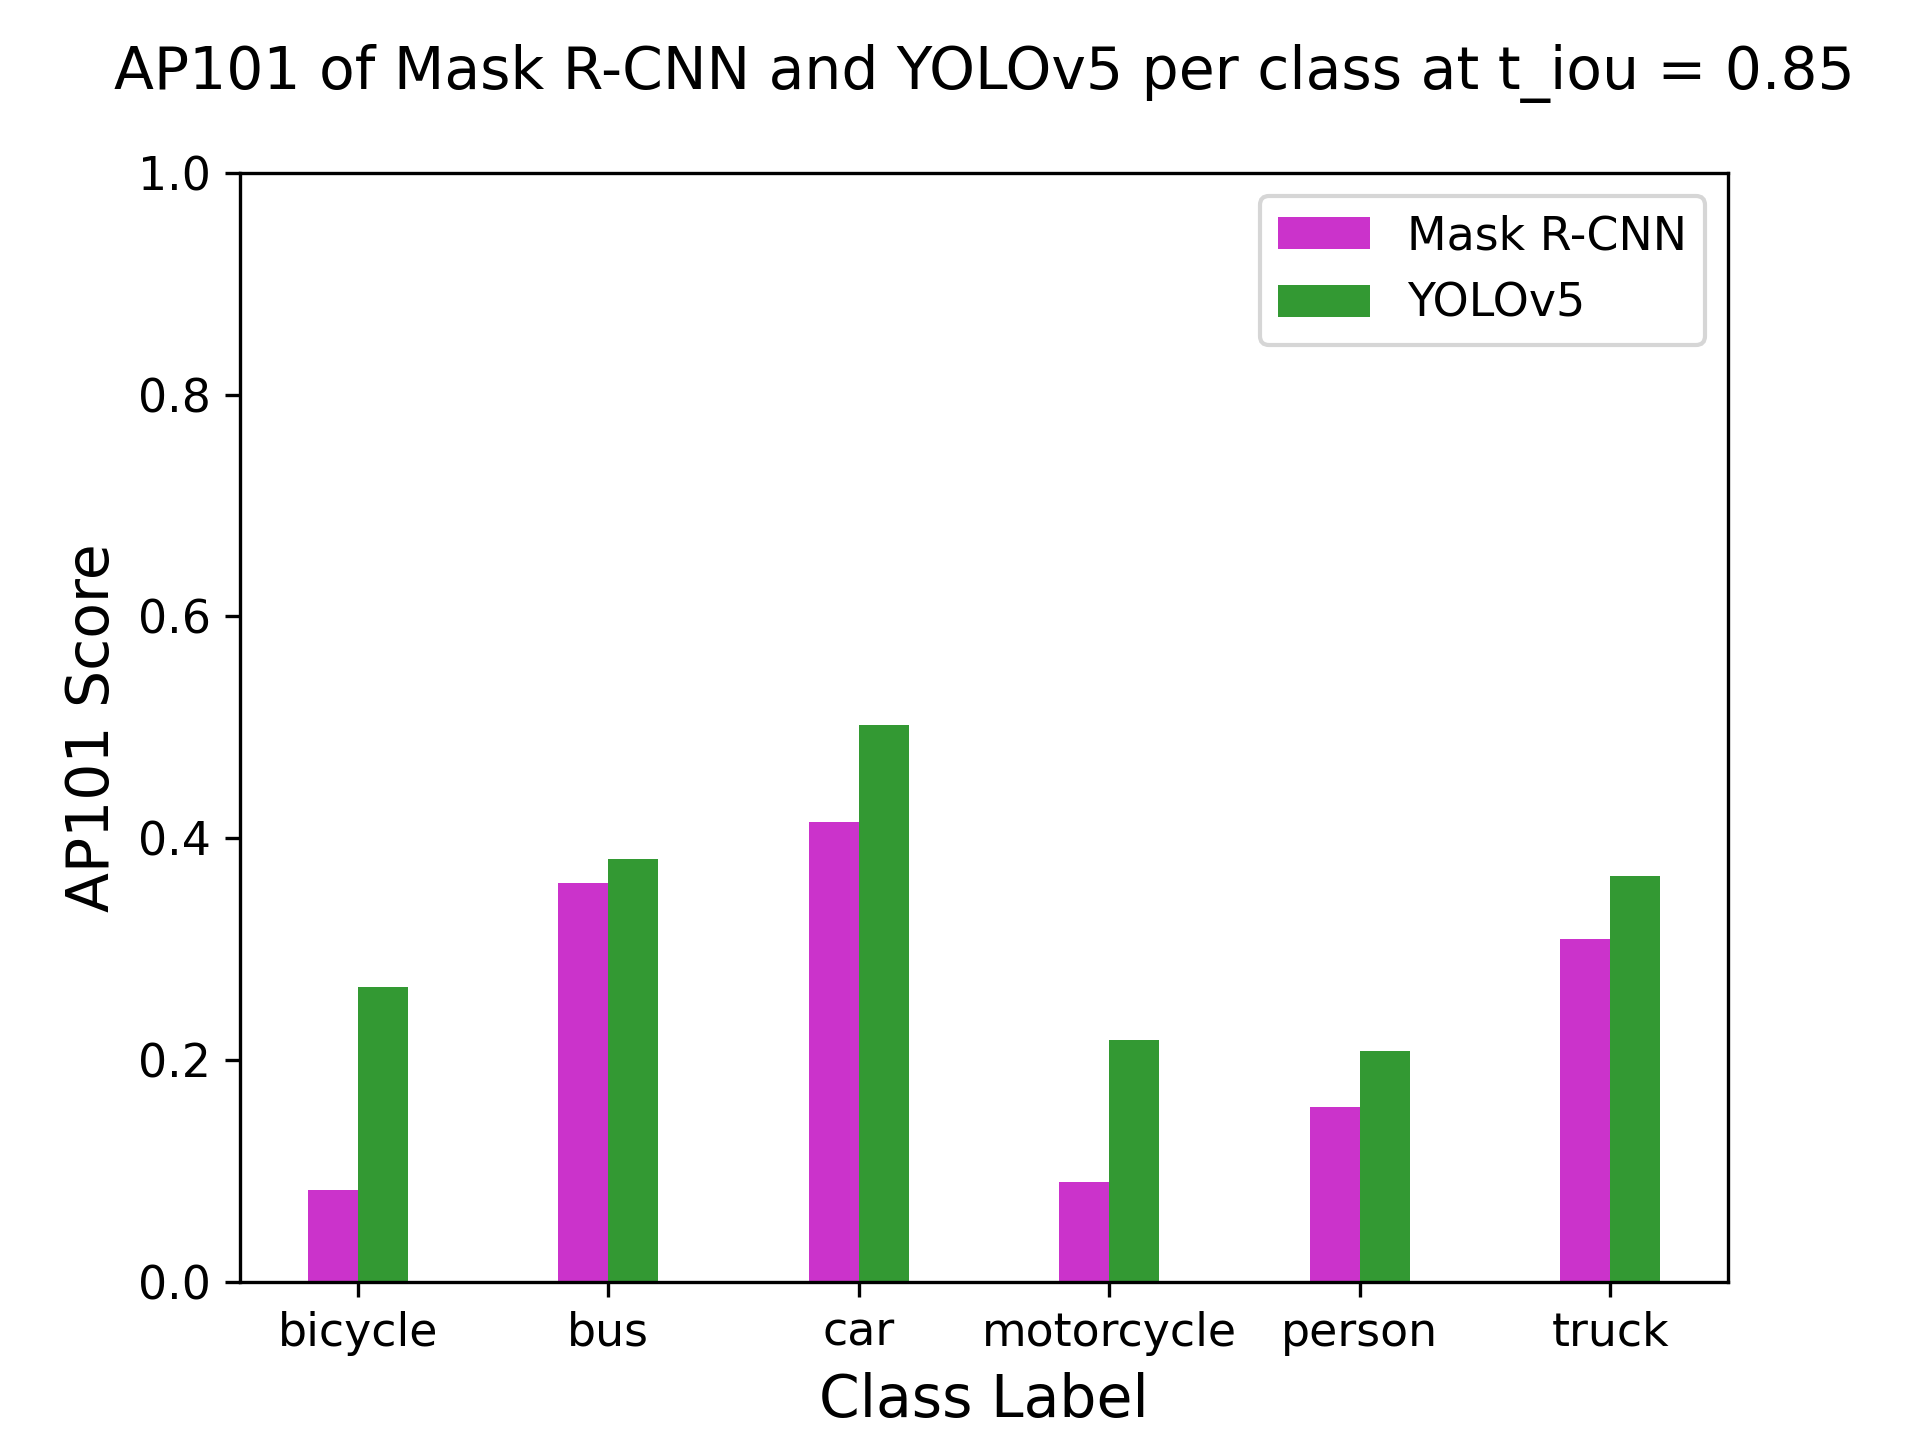
\includegraphics[height=1.5in]{figures/ap101_i85.png}
    }
    \caption{$AP_{101}$ score of Mask R-CNN and YOLOv5 model for each supported label at IoU thresholds of 0.55, 0.65, 0.75, and 0.85} 
    \label{fig:ap101_perlabel_periou}
\end{figure}

\begin{figure}[!ht]
    \centering
    \subfloat[][True Positive at IoU threshold of 0.5 and confidence threshold of 0.5]{
        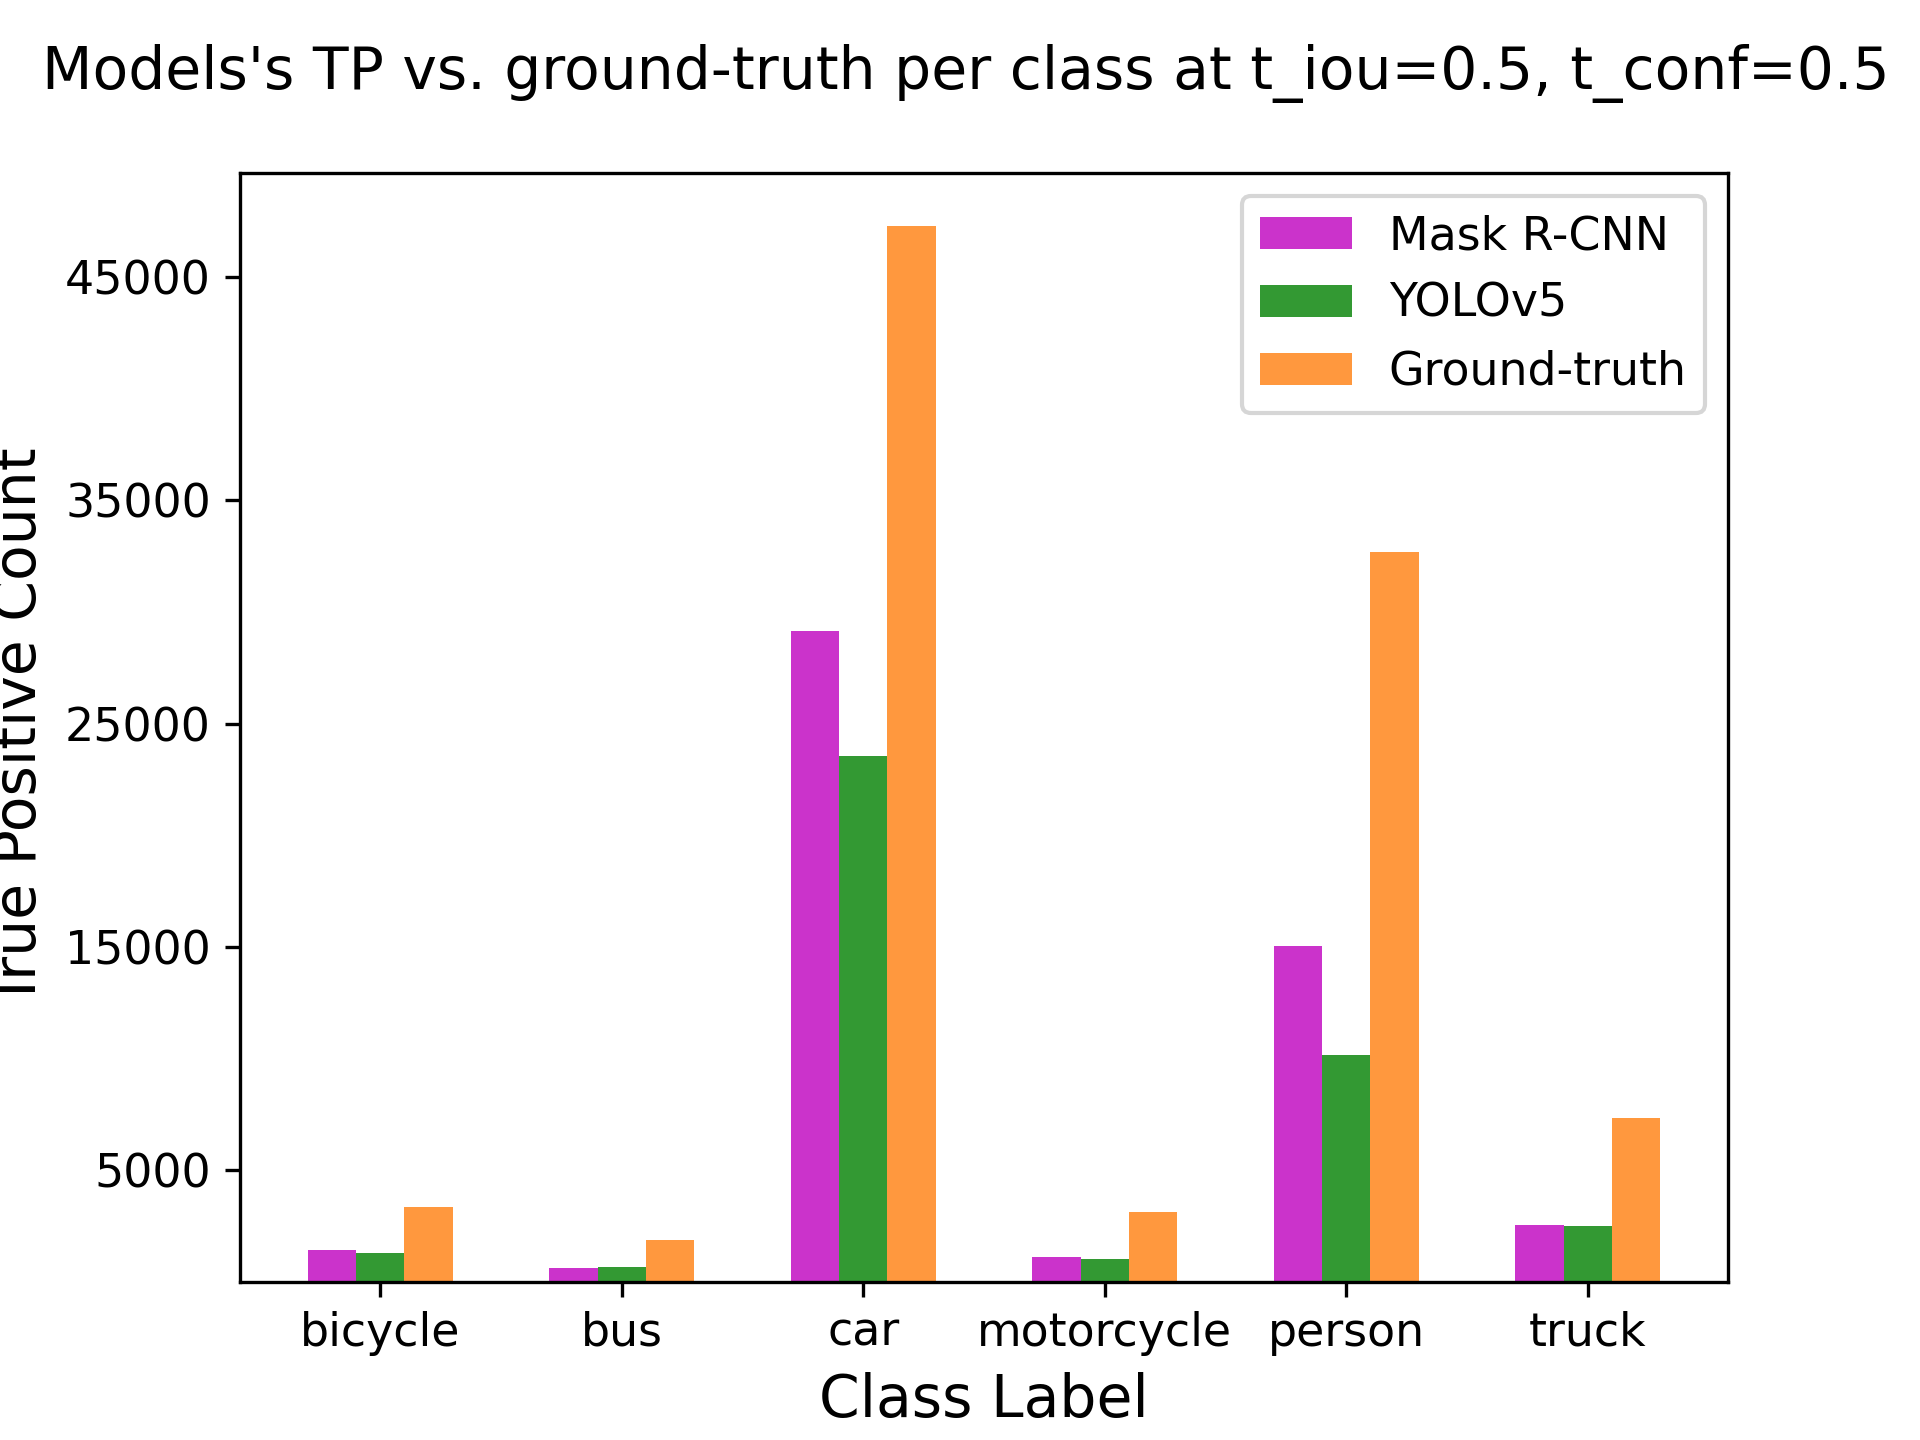
\includegraphics[height=1.5in]{figures/tp_i50_c50.png}
    }
    \quad
    \subfloat[][True Positive at IoU threshold of 0.85 and confidence threshold of 0.5]{ 
        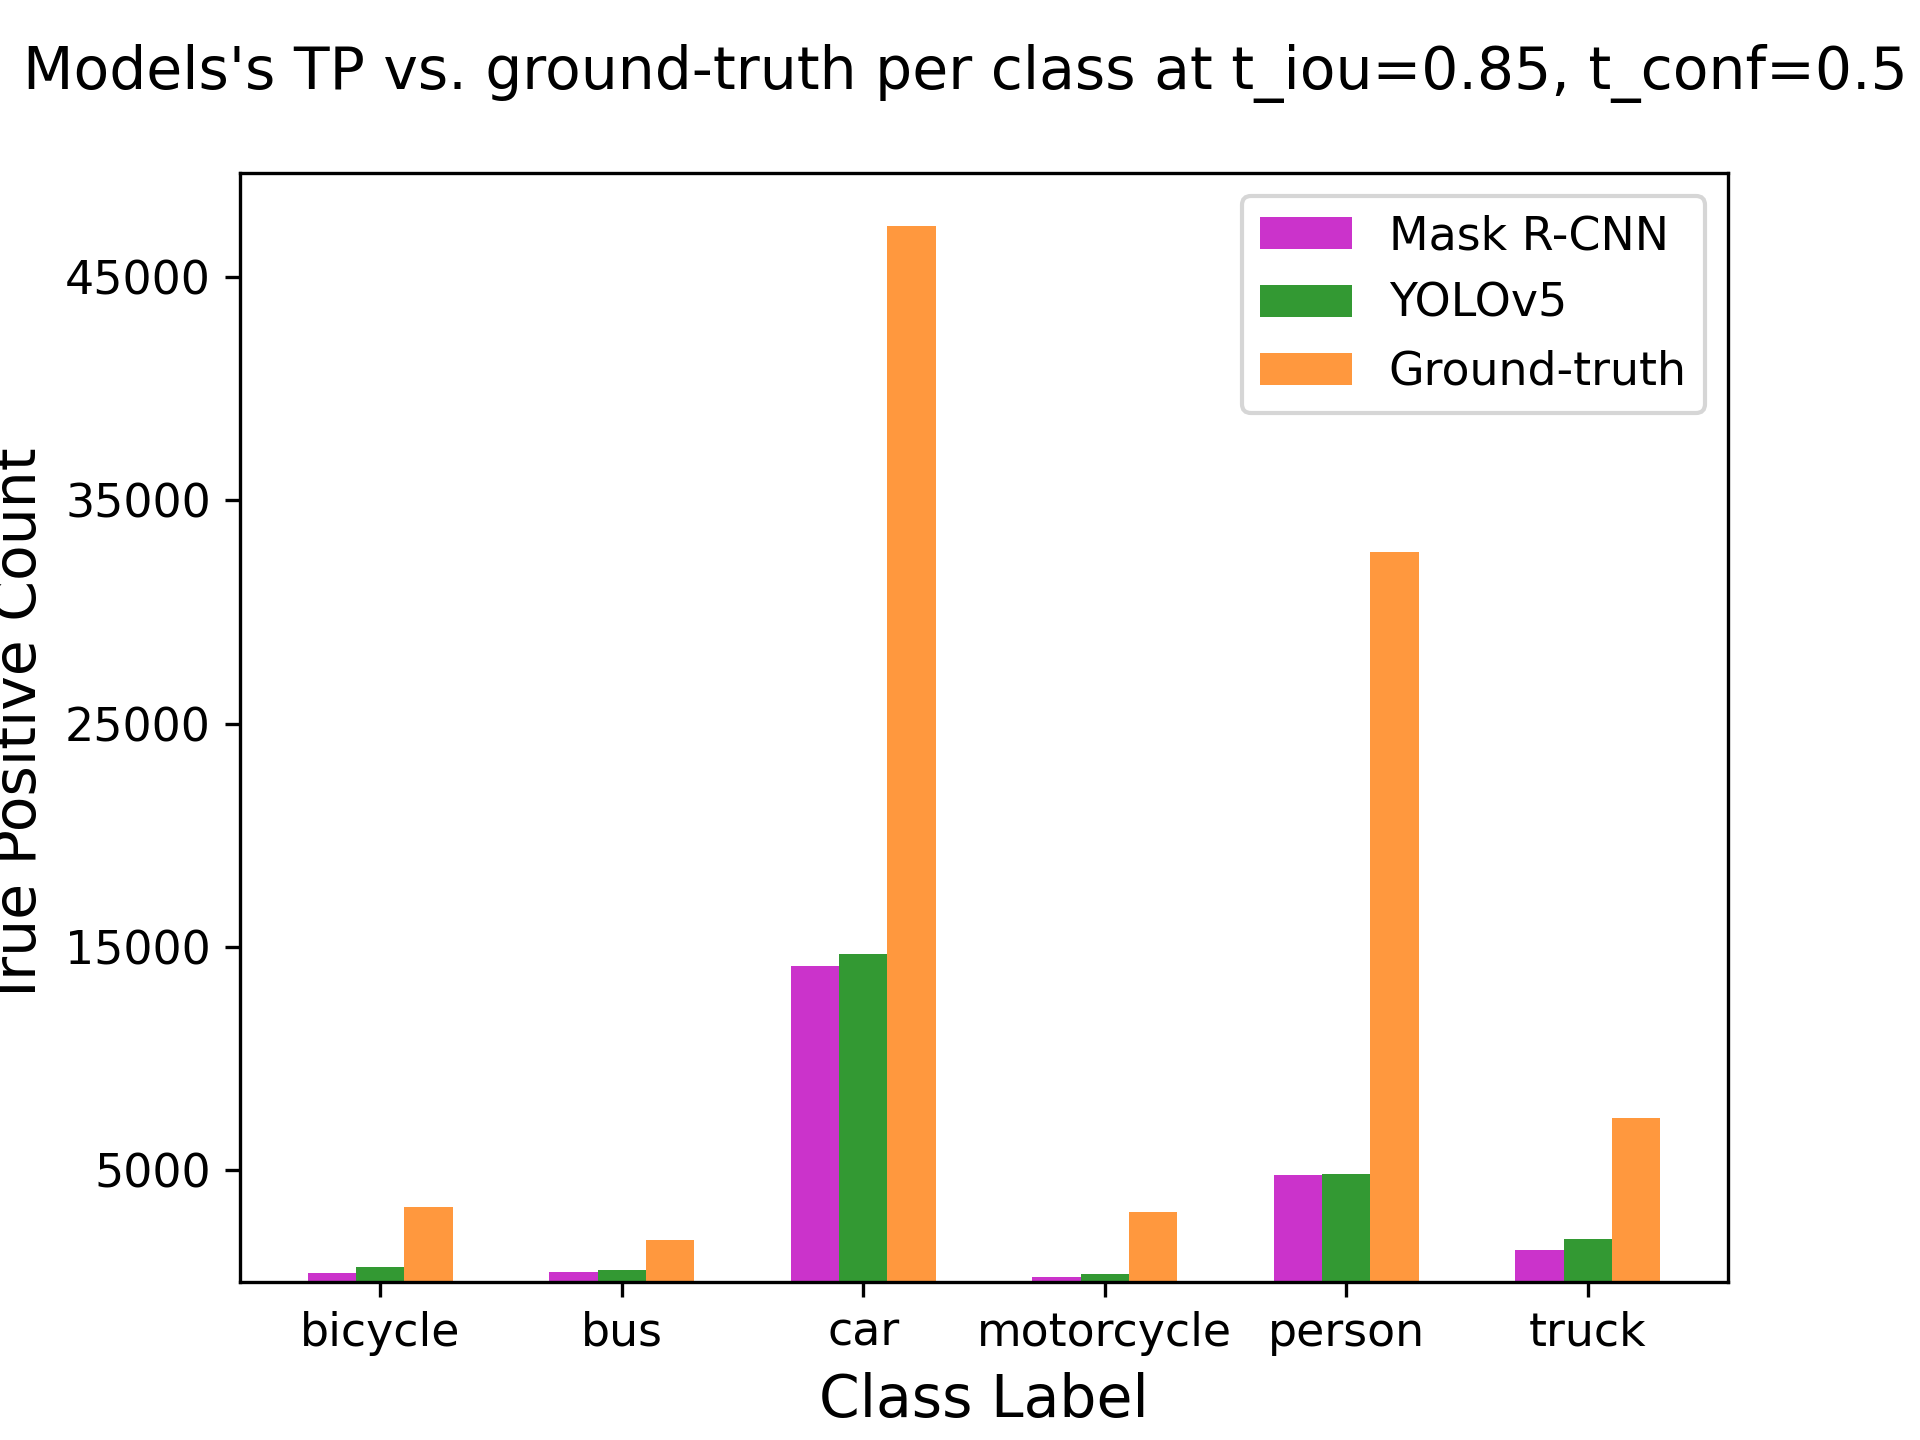
\includegraphics[height=1.5in]{figures/tp_i85_c50.png}
    }
    \caption{Number of detected objects by Mask R-CNN and YOLOv5 versus the number of ground-truth objects. The comparisons are at IoU thresholds of 0.5, 0.85, and the confidence threshold of 0.5. The comparison is displayed for each supported label.} 
    \label{fig:model_missed_detection}
\end{figure}